\documentclass[conference]{IEEEtran}

% 4 oder 8 Seiten

\IEEEoverridecommandlockouts

\usepackage{cite}
\usepackage[pdftex]{graphicx}

\ifCLASSOPTIONcompsoc
  \usepackage[caption=false,font=normalsize,labelfont=sf,textfont=sf]{subfig}
\else
  \usepackage[caption=false,font=footnotesize]{subfig}

\usepackage[bookmarks=false]{hyperref}

\hyphenation{}

\newcommand{\citep}{\cite}

\begin{document}

\title{Actor Based Business Process Modeling and Execution: a Reference Implementation Based on Ontology Models and Microservices}

\author
{
\IEEEauthorblockN{
	Matthias Geisriegler$^*$, Maksym Kolodiy$^*$, Stefan Stani$^*$, and Robert Singer$^\dagger$}
\IEEEauthorblockA{
	FH JOANNEUM -- University of Applied Sciences\\
	Dep. of Applied Computer Sciences\\
	Alte Poststra\ss e 147\\
	8020 Graz, Austria\\
	robert.singer@fh-joanneum.at}
\thanks{$^*$Equal contribution}
\thanks{$^\dagger$Corresponding author}
%\thanks{$^*$Equal contribution}
%\thanks{$^\dagger$Corresponding author}
}

\maketitle

\begin{abstract}
text  
\end{abstract}

\IEEEpeerreviewmaketitle

\section{Introduction}
\label{Introduction}

Current developments in business, the demand for digitalization, and technology driven new business models foster more than ever the need for mature business process management (BPM) methodologies and corresponding supporting technologies for distributed business processes, so-called choreographies. Communication is the very nature of a business process choreography---or, in other words, any choreography is a set of structured communication patterns. That means a choreography defines how work is done, taking into account all involved process participants and systems.

During recent years, tools have emerged to support the execution of business processes, so-called Business Process Management Suits (BPMS). Most of these tools are built around the \emph{de facto} standard for business process modeling languages, namely Business Process Model and Notation (BPMN 2.x).

The standard may be suitable for modeling purposes, but does not directly support the execution of business process models~\citep{OMG:2013wz}\citep{Silver.2011}\citep{Borger:2011ib}. That means, there is a gap between the conceptual model and the digitized and executable representation. For example, the BPMN standard document provides several compliance classes. Though, the class for execution offers only a rather restricted subset of the modeling classes and no execution support for process collaborations and choreographies~\cite{OMG:2013wz}. 

To overcome this weakness, modeling notations based on actor models have emerged. The standard for an actor based approach for business process modeling is the so-called Subject-oriented Business Process Management (S-BPM) approach~\citep{Fleischmann:2012va} which not only provides a formal but rather simple, modeling notation and also allows a direct translation into executable code. S-BPM is a mature approach, as has been proven in theory and practice~\citep{Fleischmann:1994wf}\citep{Fleischmann:2012va}\citep{Fleischmann:2013vm}\citep{Fleischmann:2015}. 

In this paper, we will discuss how to move away from monolithic software suites towards agile approaches. The central research question is, how to define a BPMS architecture which is fully based on microservice design principles.

To have a common understanding, we will shortly discuss some topics for a shared understanding of the problem domain. Then we will discuss an architecture based on microservice for the execution of process models; the discussion builds on a prototypical implementation of the presented architecture, which is also available for further research. We will not argue why in this case a software architecture based on microservices is more adequate than a monolithic one; we take this for granted and as state of the art for enterprise applications~\cite{Amundsen:2016}\cite{Newman:2015ye}.

\section{Workflow Systems}
\label{traditionalworkflowsystem}	

A typical conceptual architecture of an enterprise workflow system as part of a business process management system is based on a monolithic architecture, as described in~\citep{Hollingsworth:1994}, for example. All known workflow-engines are based on these architectural concepts; therefore, most of them are heavyweight applications with steep learning curves. Moreover, many of these applications have "problems" to realize process collaborations in a practical way. This can easily be proved by trial and is rooted in the underlying concept to conceptualize a business process as \textit{one} finite state machine (FSM).

\section{Subject-oriented Business Process Management (S-BPM)} 

\section{S-BPM Execution Platform}
\label{ExecutionPlatform}

\subsection{Previous Work}
Previously we have presented an entirely functional S-BPM workflow solution\footnote{https://github.com/InFlowBPM/InFlow-BPMS} using the Microsoft Windows Workflow Foundation functionality as discussed in~\citep{Singer:2014} and~\citep{Singer:2015}. The designed architecture has full enterprise functionality and supports the execution of inter- and intra-company business processes (i.e. collaborations, choreographies).

Nevertheless, the developed prototype is still based on the concepts of traditional workflow systems---e.g. \textit{one} web server for all process instances--- and needs many infrastructure components as a functional backbone and is therefore rather costly and has a rather high complexity.

\subsection{Prototype based on Microservices}

One major design goal of our architecture is to separate the modeling and the execution platform. As a result, the modeling platform generates an OWL file that can be uploaded to the execution platform by using the management user interface (UI). The management UI provides an interface to control the execution of processes. The individual platforms are based on different sets of technology, as will be described next.

\begin{figure}
	\centering
	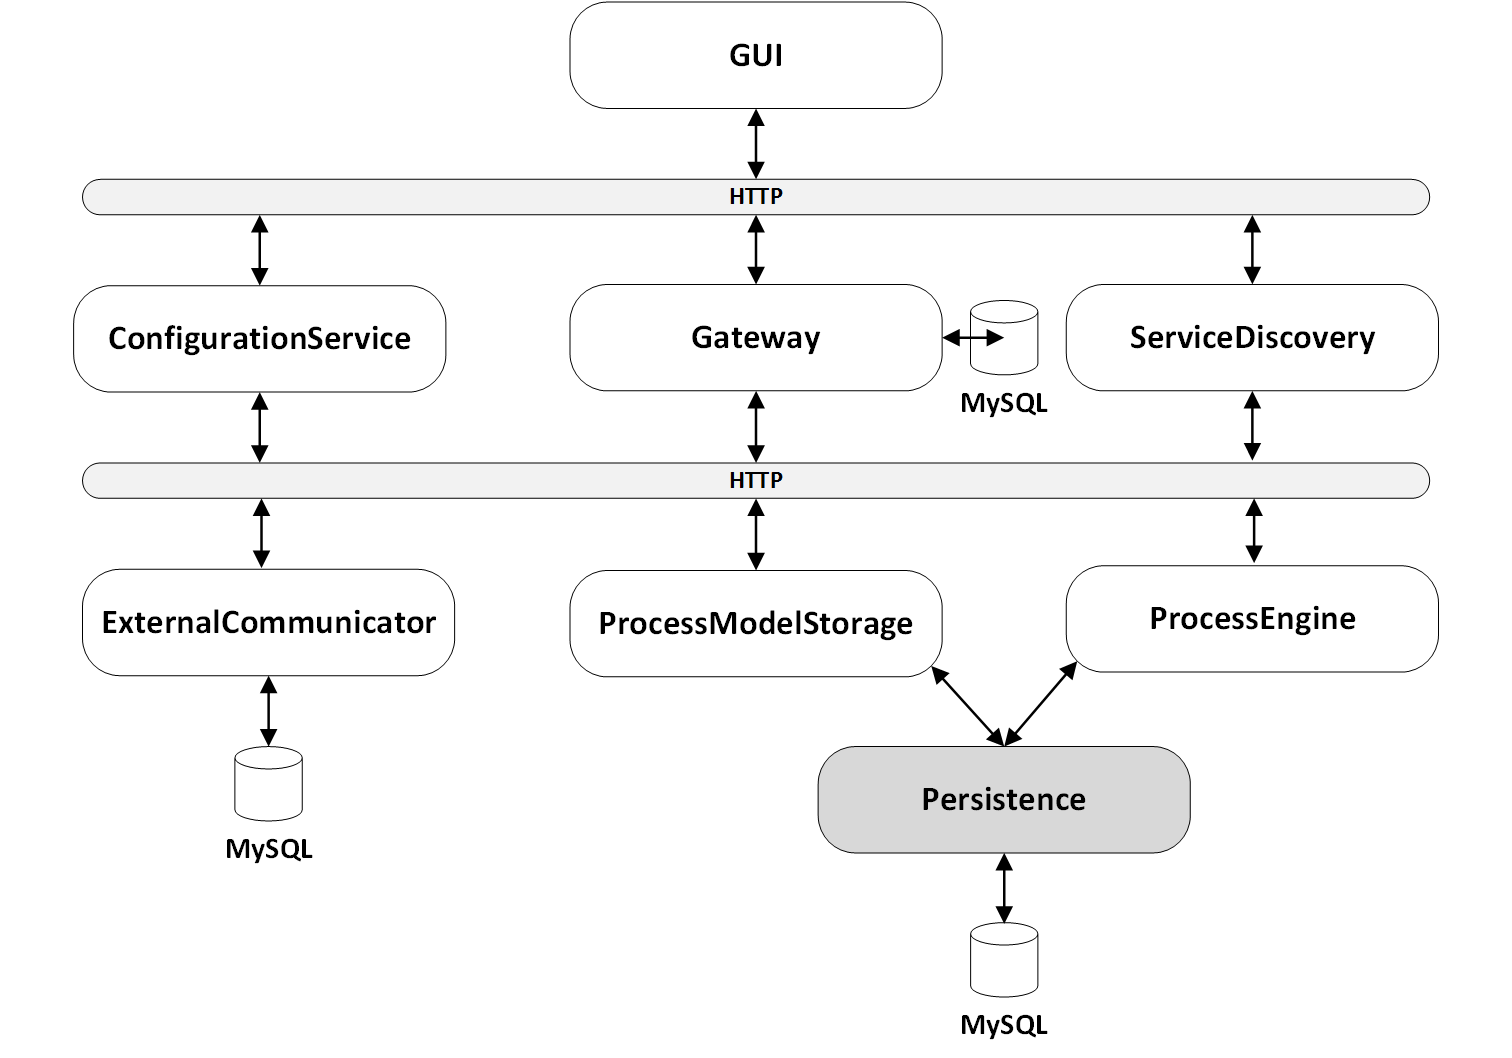
\includegraphics[keepaspectratio,width=8.5cm,height=0.75\textheight]{fig-1.png}
	\caption{The architecture of the prototype: a collection of microservices.}
	\label{architecture}
\end{figure}

\subsubsection{Graphical User interface (GUI)}

\subsubsection{Configuration Service}

\subsubsection{Gateway}

\subsubsection{Service Discovery} 

\subsubsection{ExternalCommunicator}

\subsubsection{ProcessModelStorage}

\subsubsection{ProcessEngine}

The ProcessEngine is the most extensive service of the execution platform. This service provides features to start, stop processes, and handles the complete workflow of processes. The Process Engine is based on Akka, which is one of the most popular Actor Model frameworks. 

In the Actor Model, all objects are independent, computational units. These units only respond to received messages and do not share a common state. Actors change their state only when they receive a stimulus in the form of a message. So, an actor is a computational entity that, in response to a message it receives, can concurrently~\citep{Gupta:2012}:

\begin{itemize}
	\item send a finite number of messages to other actors
	\item create a finite number of new actors
	\item designate the behavior to be used for the next message it receives
\end{itemize}


\section{Modeling Platform}
\label{ModelingPlatform}


\section{Discussion} 

With this prototype, we want to stimulate further research in the domain of business process modeling and execution (the prototype is released as open source software). The presented and discussed architecture (which is still under development at the time of writing) is a starting point to define a modern reference architecture for BPMS which are based on microservices. 

The microservice approach supports several real requirements for enterprise software: with this work, we have a proof of concept, which demonstrates the practical usability of the microservice approach in the domain of business process management, in concrete in the development of agile workflow systems. Nevertheless, the pre-condition to building an agile BPMS is to change the way how to define process models.

\bibliographystyle{IEEEtran}
\bibliography{SEAAnew}

\end{document}
